
\title{Sistemi Informativi \\ Laboratorio 5}
\author{
        Catalin Copil
            \and
        Mattia de Stefani
            \and
        Giulio Lovisotto
}
\date{\today}

\documentclass[12pt]{article}
\usepackage{algorithmicx}
\usepackage{algpseudocode}
\usepackage{graphicx}
\usepackage{geometry}

\addtolength{\topmargin}{-.5in}
\begin{document}
\maketitle

\section{Descrizione}
Computeremo il \textsc{pagerank} con la libreria \texttt{networkx} a tempo di indexing e salveremo i risultati su un file ($id \rightarrow pagerank$). La nostra funzione di reperimento combinera' gli score di BM25 ($rk$) con pagerank ($pr$) nel seguente modo:

\[ score =  \alpha \cdot rk + (1-\alpha) \cdot pr,\]

dove $\alpha$ e' un parametro tra 0 e 1 che determina l'importanza del ranking (primo termine) e del pagerank (secondo termine). 

Per poter confrontare in modo coerente il pagerank e lo score di BM25, abbiamo deciso di ridimensionare entrambe le distribuzioni, normalizzando in modo da avere valori tra 0 e 1. Abbiamo usato la seguente formula:

\[ z_i = \frac{x_i - min(x)}{max(x) - min(x)}, \]

Dopo la normalizzazione, al variare di alpha tra 0 e 1 il peso viene spostato uniformemente da pagerank a BM25.

\section{Implementazione}
Per calcolare il pagerank, abbiamo usato la libreria \texttt{networkx}. Tale libreria permette di costruire il grafo delle citazioni a partire dalla lista di archi con il metodo \texttt{read\_edgelist}. Permette inoltre di computare il pagerank con il metodo \texttt{pagerank}, che usa \textit{power iteration} sulla matrice di transizione.

Pagerank viene computato a tempo di indexing, e i valori vengono salvati su un file che verra' usato a tempo di retrieval.

\section{Risultati}
Abbiamo provato diversi valori per $\alpha$. Riportiamo in Figura \ref{fig:uno} i risultati di Mean Average Precision.

\begin{figure}[htbp]
\begin{center}
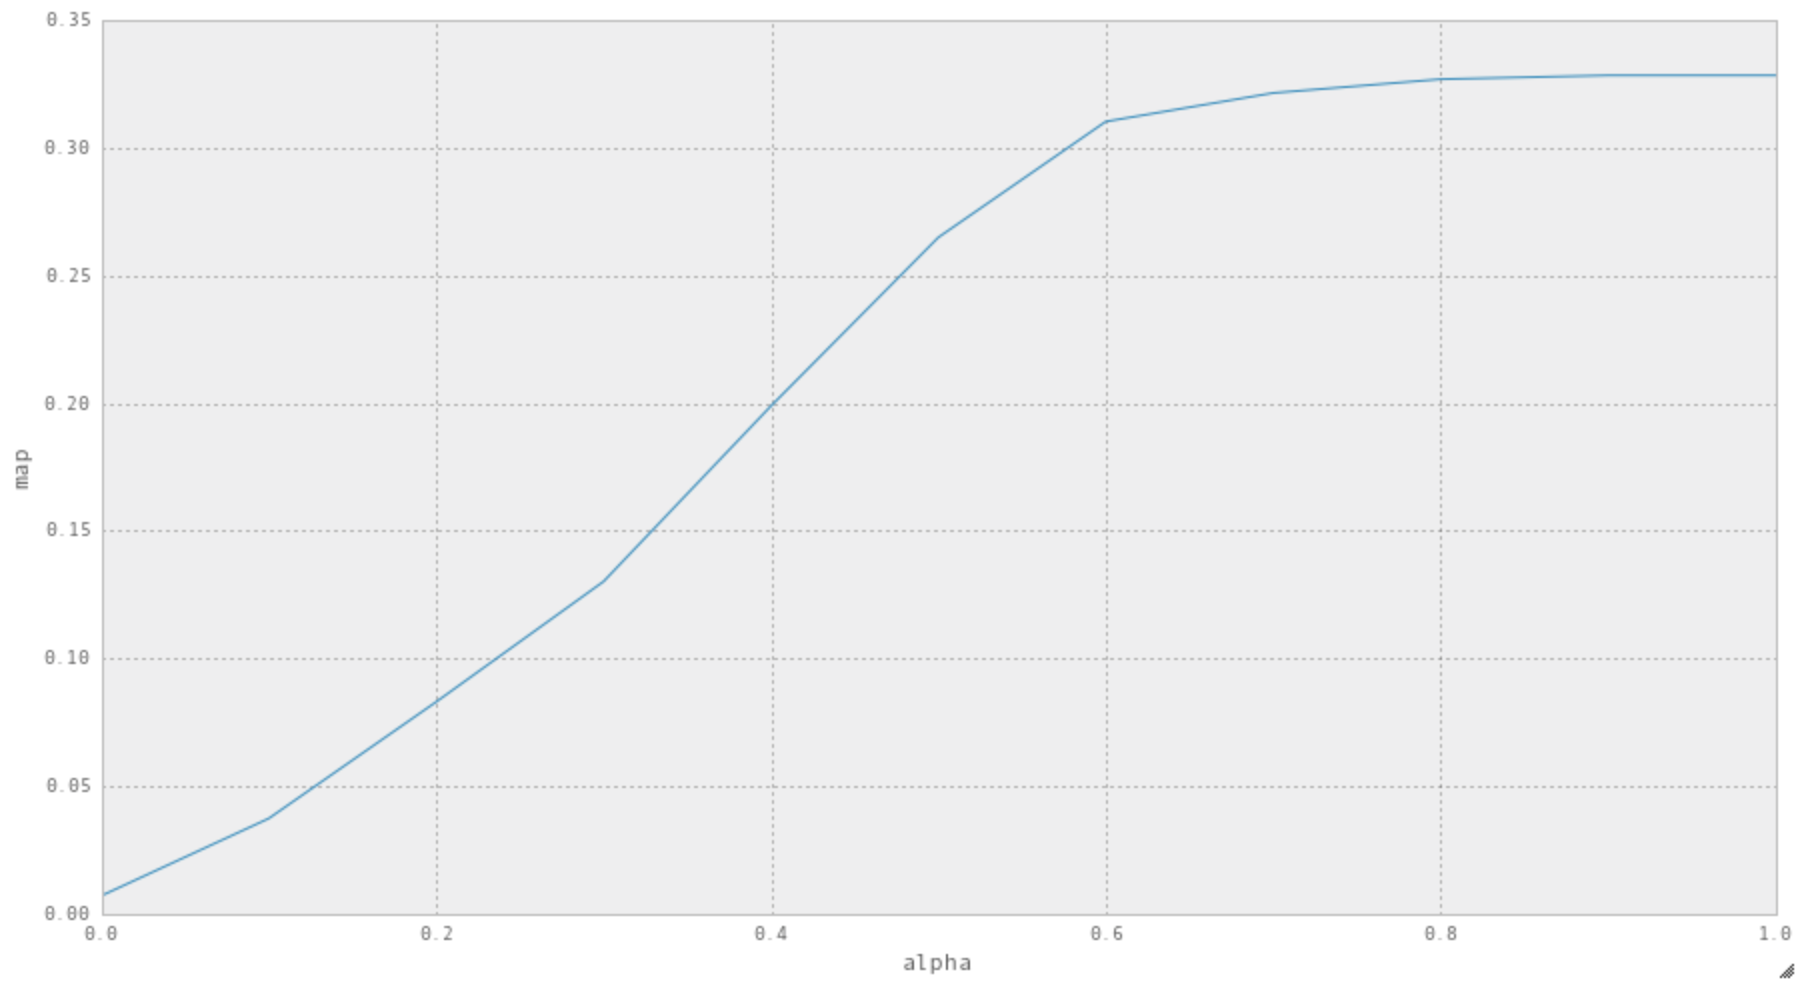
\includegraphics[width=0.9\textwidth]{map.png}
\caption{Risultati \textit{trec\_eval} per vari valori di $\alpha$.}
\label{fig:uno}
\end{center}
\end{figure}

Come si evince dal grafico, per $\alpha =1$, che significa non considerare la componente pagerank nello scoring, otteniamo la migliore precisione $map$. Cio' significa che il pagerank nella nostra collezione non e' davvero informativo, probabilmente perche' ci sono molti documenti che non hanno citazioni.

Il file \texttt{G12R9PR.txt} contiene i risultati ottenuti utilizzando $\alpha = 0.9$.

\bibliographystyle{abbrv}
\bibliography{main}

\end{document}